\documentclass[tikz]{standalone}
\usepackage{pgfplots}
\usepackage[left=2.5cm,right=2.5cm,top=3cm,bottom=3cm]{geometry}
\usetikzlibrary{patterns}

\begin{document}
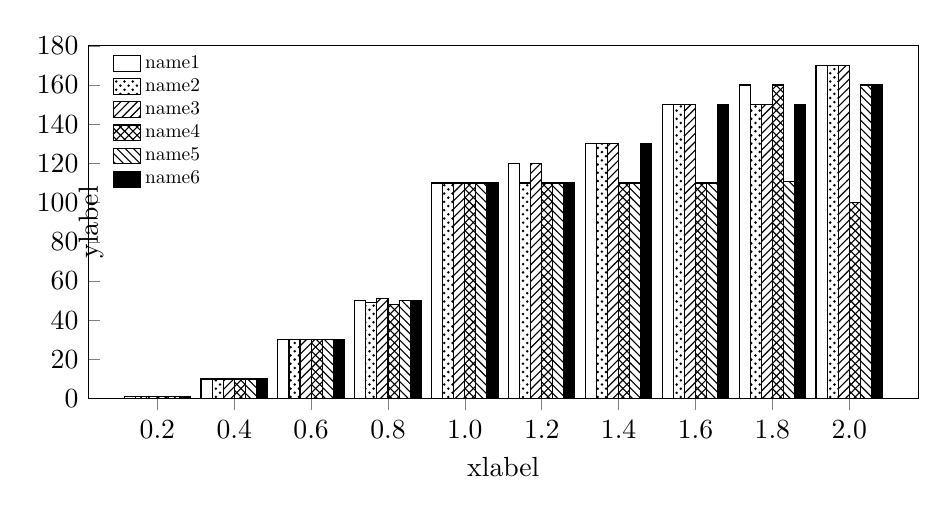
\begin{tikzpicture}
\pgfplotstableread{
budget    name1   name2   name3   name4    name5    name6
0.2 1   1   1   1   1   1
0.4 10  10  10  10  10  10
0.6 30  30  30  30  30  30 
0.8 50  49  51  48  50  50
1.0 110 110 110 110 110 110
1.2 120 110 120 110 110 110
1.4 130 130 130 110 110 130
1.6 150 150 150 110 110 150
1.8 160 150 150 160 111 150
2.0 170 170 170 100 160 160
}{\datatable}
\begin{axis}[
    width = \linewidth, height = 0.5\linewidth,
    %title={The Title},
    title style={at={(0.5,-0.35)}},
    xtick pos=bottom,
    ytick pos=left, % remove the tick from the right and top
    ybar=0,
    ylabel={ylabel},
    ylabel style={at={(axis description cs:0.03,0.5)}},
    ytick={0,20,...,180},
    bar width=4pt,
    %enlarge x limits=0.15,
    ymin=0, ymax=180,
    % legned related -------------
    legend image code/.code={
        \draw [#1] (0cm,-0.1cm) rectangle (0.35cm,0.1cm);
    },
    legend style={
        at={(0.15,1)},
        nodes={scale=0.7},
        draw = none,        % without box
        cells={anchor=west}, % algin left
    },
    xlabel={xlabel},
    % xtick related 
    xtick=data,
    xticklabels from table={\datatable}{budget},
    %xticklabel style={
    %j    rotate=45,xshift=-100,yshift=-100,anchor=mid east
    %j},
    ] % end of options of axis environment

\newcommand{\mysubplot}[2]{
    \addplot[#2] table [x=budget,y=#1] {\datatable};
    \addlegendentry{#1};
}
\mysubplot{name1}{}
\mysubplot{name2}{pattern=crosshatch dots}
\mysubplot{name3}{pattern=north east lines}
\mysubplot{name4}{pattern=crosshatch}
\mysubplot{name5}{pattern=north west lines}
\mysubplot{name6}{fill=black}

\end{axis}
\end{tikzpicture}
\end{document}